\subsubsection*{Problem definition}

The aim of this example is to simulate the transport of several components with different sorption behaviour and decay. The calculation area and boundary conditions are the same as described for the precedent example. The mass distribution after 100 days has to be calculated.

\textsl{Assumptions}

\begin{tabbing}
Component 1: \= no sorption, no decay \\
Component 2: \> decay \\
Component 3: \> linear sorption \\
Component 4: \> linear sorption, decay \\
Aquifer: \> homogeneous, saturated, stationary flow \\
\end{tabbing}

\subsubsection*{Model set-up of the 1~D numerical model}

See chapter \ref{sec:decay}

The soil parameters are the same as listed in table \ref{tab51}. The decay rate $\lambda$ for components 2 and 4 is 2$\cdot 10^{-7}$~s$^-1$, the Henry sorption coefficient K$_D$ for component 3 is 6.4$\cdot 10^{-4}$~kg/m$^-3$ (R = 6.44).

\subsubsection*{Evaluation method}
The concentration distribution at a special point in time and over a given distance is calculated by equation \ref{eq9}. The analytical solutions are depicted in figure \ref{fig59} as single symbols.

\subsubsection*{Results}

In figure \ref{fig59} you can find the concentration distribution of the 4 different components over the whole length of the 1D-model at the final simulation time of 100 days. As the comparison of each single component with the analytical results of the "one-component-transport" shows, the numerical results for the multi component transport are reasonable.

\begin{figure}[htbp]
\centering
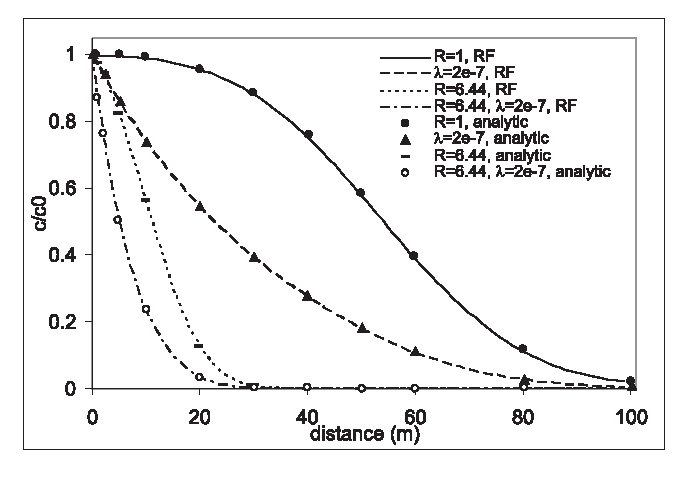
\includegraphics[width=0.5\textwidth]{C/figures/fig59.eps}
\caption{Concentration distributions of the four components after 100~d}
\label{fig59}
\end{figure}


\begin{tabular}{|l|l|l|l|}
\hline
Path in the & Used code	& Used version & Date of si- \\
benchmark deposit	& & & mulation run \\
\hline
$\backslash$HC$\backslash$multi\_component$\backslash$ &Rockflow	& RockFlow 5,	& Mar. 2007 \\
hc\_multi-c\_1D.rfd/rfi	&  & rf\_gui1407-rf5065 & \\
\hline	
\end{tabular}
